\section{Lecture 11}
\subsection{Computing Real Integrals with Residues - Continued}

\begin{example}
The Fresnel Integrals are the real and imaginary parts of the following integral:
\[I = \int_0^\infty e^{-ix^2} dx\]
How does one compute $I$?
\end{example}

\begin{proof}[Answer]
We will first look at the Gaussian Integral, which we are quite familiar with already:
\[\int_{0}^\infty e^{-x^2} dx = \frac{\sqrt{\pi}}{2}\]
Now for the Fresnel Integrals, consider the following contour:
\[\fbox{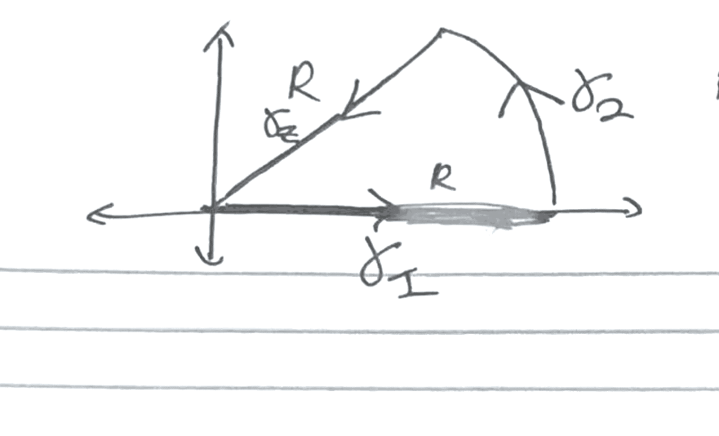
\includegraphics[width=.5\textwidth]{Figures/contour-7.png}}\]
We note that $e^{-iz^2}$ is analytic over the entire region, so Cauchy's Integral Theorem tells us that
\[0 = \int_{\gamma_1} e^{-iz^2} dz + \int_{\gamma_2} e^{-iz^2} dz + \int_{\gamma_z} e^{-iz^2} dz \]
We note that as $R \to \infty$, a similar argument as before show that the integral over $\gamma_2$ vanishes. Thus, we have that
\[I = \lim_{R \to \infty} \int_{\gamma_1} e^{-iz^2} dz = -\lim_{R \to \infty} \int_{\gamma_z} e^{-iz^2} dz\]
We can parameterize $\gamma_3$ as $z = \frac{1 + i}{\sqrt{2}} t$ from $t = R$ to $t = 0$, then
\begin{align*}
    \int_{\gamma_z} e^{-iz^2} dz &= \int_R^0 e^{-t^2} \frac{1 + i}{\sqrt{2}} dt\\
    &= -\frac{1 + i}{\sqrt{2}} \int_0^R e^{-t^2} dt\\
    \lim_{R \to \infty} \int_{\gamma_z} e^{-iz^2} dz &= -\frac{1 + i}{\sqrt{2}} \int_0^\infty e^{-t^2}\\
    &= -\frac{1 + i}{\sqrt{2}} \cdot \frac{\sqrt{\pi}}{2}
\end{align*}
\end{proof}

\subsection{Argument Principle}

Let $G$ be a bounded domain and $\partial G \in PC^1$, and consider points $p_1, ..., p_m \in G$. Suppose $f \in Hol(cl(G) \setminus \{p_1, ..., p_m\})$, meaning that $f$ is holomorphic in $\Omega \setminus \{p_1, ..., p_m\}$ where $\Omega$ is an open set containing $cl(G)$.\\

Suppose furthermore that $f(z)$ is not the constant zero function. We note that $cl(G)$ is compact, so the asusmption above implies that $f$ has finitely many zeroes in $cl(G)$. Otherwise, if $f(z)$ has infinitely many zeroes, compact sets are sequentially compact in $\Cbb$, so $f$ would containing some zero that's not isolated, violating the Uniqueness Theorem. Let $z_1, ..., z_N$ be the zeroes of $f(z)$.\\

Now assume that $f(z) \neq 0$ for all $z \in \partial G$, the Argument Principle states that:

\begin{theorem}[Argument Principle]
Let $Z$ be the number of zeros inside $G$ (counting order of the zero) and $P$ be the number of poles inside $G$ (counting order of the pole), then
\[Z - P = \frac{1}{2\pi i} \int_{\partial G} \frac{f'(z)}{f(z)} dz\]
\end{theorem}

\underline{\textbf{Note that when we say number of zeroes, we are always counting multiplicity.}}

\begin{proof}
We first note that $\frac{f'(z)}{f(z)}$ is not holomorphic on a given $z$ if and only if $z$ is one of the poles or the zeros of $f(z)$.\\\\
Since $f$ is analytic, take $a \in cl(G)$, let $f(z) = (z - a)^m g(z)$ where $g(a) \neq 0$, then we note that
\begin{align*}
    \frac{f'(z)}{f(z)} &= \frac{m(z - a)^{m-1} g(z) + (z-a)^m g'(z)}{(z - a)^m g*z(}\\
    &= \frac{m}{z - a} + \frac{g'(z)}{g(z)}
\end{align*}
Since $g(a) \neq 0$, we note that $\frac{g'(z)}{g(z)}$ is analytic in a neighborhood of $a$ and can be represented as a power series, so
\[\frac{f'(z)}{f(z)} = m(z - a)^{-1} + \sum_{n = 0}^\infty b_n (z - a)^n\]
Thus, in other words, $m$ is the coefficient of the $-1$-th power term, hence
\[res(\frac{f'(z)}{f(z)}, a) = m\]
If $a$ is one of the zeroes $z_k$, then $m$ is exactly the order of the zero.\\\\
If $a$ is one of the poles $p_k$, then $m$ is given by factoring out the Laurent Series. Clearly $m$ is exactly $-1$ times the order of the pole.\\\\
Thus, applying Residue's Theorem around the zeroes and the poles, we have that
\[Z - P = \frac{1}{2\pi i} \int_{\partial G} \frac{f'(z)}{f(z)} dz\]
\end{proof}

\begin{remark}
Why is this theorem called the \textbf{Argument Principle}? This is because $\frac{f'(z)}{f(z)}$ is actually primitive given a chosen branch, and
\[\frac{f'(z)}{f(z)} = [\log f(z)]'\]
Thus, often we sometimes rewrite the Argument Principle as
\[Z - P = \frac{1}{2\pi i} \int_{\partial G} d \log(f(z))\]
We claim that in fact
\[\frac{1}{2\pi i} \int_{\partial G} d \log(f(z)) = \frac{1}{2\pi} \int_{\partial G} d(\arg f(z))\]
\end{remark}

\begin{proof}
We first note that we can rewrite $f(z)$ in its polar coordinate form as
\[f(z) = r(z) e^{i \cdot arg(f(z))}\]
, then we have that
\begin{align*}
    \frac{1}{2\pi i} \int_{\partial G} d \log(f(z)) &= \frac{1}{2\pi i} \int_{\partial G} d(\log[r(z)e^{i \cdot arg(f(z))}])\\
    &= \frac{1}{2\pi i} \int_{\partial G} d(\log r(z)) + \frac{1}{2\pi i} \int_{\partial G} i \cdot d(arg(f(z)))\\
    &= \frac{1}{2\pi i} \int_{\partial G} d(\log r(z)) + \frac{1}{2\pi} \int_{\partial G} d(\arg f(z))
\end{align*}
It remains for us to show that $\frac{1}{2\pi i} \int_{\partial G} d(\log r(z))$ is actually $0$. We first note that by the Argument Principle, this integral is an integer. Now, since $r(z)$ is a real valued function, $\int_{\partial G} d(\log r(z))$ is real, hence the integral is also a complex number.\\\\
The only number that is both complex and integer is $0$.\\\\
Thus, we conclude that
\[\frac{1}{2\pi i} \int_{\partial G} d \log(f(z)) = \frac{1}{2\pi} \int_{\partial G} d(\arg f(z))\]
\end{proof}

\subsection{Rouche's Theorem}

Rouche's Theorem is a standard corollary of the Argument Principle. Assume the same setup as before:\\

Suppose $G$ is a bounded domain with $\partial G \in PC^1$ and $f, h \in Hol(cl(G))$:

\begin{theorem}[Rouche's Theorem]
Suppose that $|h(z)| < |f(z)|$ for all $z \in \partial G$, then the number of zeroes of $f + h$ in $G$ is the same as the number of zeroes of $f$ in $G$.
\end{theorem}

\begin{proof}
Let $\varphi(z) = \frac{f(z) + h(z)}{f(z)}$. We claim that the number of zeroes of $\varphi$ is the number of poles of $\varphi$ (inside $G$). This is because the common zeroes of $f(z) + h(z)$ and $f(z)$ would cancel out, while the rest would match, so we claim we could without choose $f, h$ such that they don't have any common zeroes.\\\\
Before we proceed with the rest of the proof, we will first justify why this is true. 
Now suppose $f(z) + h(z)$ and $f(z)$ have common zeroes $c_1, ..., c_m$ in $G$ (counting multiplicity). We note that their common zeroes have to be finite since $cl(G)$ is compact, so having a infinite number of zeroes would imply that both functions here are identically zero (by the uniqueness theorem).\\\\
Now $f(z) + h(z)$ and $f(z)$ have common zeroes $c_1, ..., c_m$ if and only if $f(z), h(z)$ have common zeroes $c_1, ..., c_m$.\\\\
Now we claim that in general, for $g \in Hol(\Omega)$ and $z_0 \in \Omega$ such that $g(z_0) = 0$, $\frac{g(z)}{z - z_0}$ has a removable singularity at $z_0$ (this just comes from the fact that its neighborhoods are bounded). So we can without loss view the quotient with the limit filled in as a holomorphic function on $\Omega$.\\\\
Applying this principle to $f(z)$ and $h(z)$, we have that
\[f(z) = \prod_{k = 1}^m (z - c_k) f_0(z), h(z) = \prod_{k = 1}^m (z - c_k) h_0(z)\]
, then the extraneous terms would cancel out but $f_0(r) \neq 0, h_0(r) \neq 0$ for any $r \in \{c_1, ..., c_m\}$.\\\\
Now, we write $\varphi(z) = 1 + \frac{h(z)}{f(z)}$, and note that
\[|\frac{h(z)}{f(z)}| < 1 \text{ on $\partial G$}\]
, so the values of $\varphi(z)$ are exactly values contained in $D_{1, 1}$ (the open disk centered at $1$ of radius $1$) by Triangle's Inequality. In particular we note this means that $Re(\varphi(z)) > 0$.\\\\
Therefore, we note that $Log \varphi(z)$ ($z \in \partial G$) is well-defined as we avoided the branch cut at $(-\infty, 0]$. Thus, it is a well-defined anti-derivative where
\[(Log \varphi(z))' = \frac{\varphi'(z)}{\varphi(z)}\]
, hence we have that
\[\int_{\partial G} \frac{\varphi'(z)}{\varphi(z)} = 0\]
Then by the argument principle, the number of zeroes and $\varphi$ is the same as the number of poles of $\varphi$ in $G$.
\end{proof}

\begin{corollary}[The Fundamental Theorem of Algebra]
Let $p(z) = \sum_{k = 0}^n a_k z^k$, where $a_n \neq 0$, then $p(z)$ has $n$ complex roots (counting multiplicity).
\end{corollary}

\begin{proof}
Take $G = D_{0, R}$ where $R > 0$ is big enough that
\[|a_n| R^n > \sum_{k = 0}^{n-1} |a_k| R^k\]
, we can find this $R$ because
\[\lim_{R \to \infty} \frac{\sum_{0}^{n-1} |a_k| R^k}{|a_n| R^n} = 0\]
We note that on $z \in \partial D_{0, R}$, $|a_n z^n| > |p(z) - a_n z^n|$, so we can take $f(z) = a_n z^n$ and $h(z) = p(z) - a_n z^n$.\\\\
Then we note that $a_n z^n$ has $n$-roots, so Rouche's Theorem tells us that $p(z)$ has $n$-roots.
\end{proof}

\subsection{Hurwitz Theorem}

\begin{definition}
Let $\{f_n\}$ be a sequence of functions, we say $f_n \to f$ converes normally in $G$ if for all compact $K \subset G$, $f_n$ converges to $f$ on $K$ uniformly.
\end{definition}

In this class, when we say $f_n$ converges to $f$ and $f_n$ are holomorphic on $G$, then we always mean that the convergence is normal!

\begin{proposition}
If $f_n$ are holomorphic functions on $G$ that converges to $f$ normally, then $f$ is also holomorphic on $G$. Furthermore, we have that $f_n^{(k)}$ converges to $f^{(k)}$ normally.
\end{proposition}

\begin{proof}
Let $R$ be a rectangle contained in $G$, since $f_n$ converges to $f$ normally, $f_n$ converges to $f$ uniformly on $R$, so we can switch the integral and limit to see that
\[0 = \lim_{n \to \infty} \int_{\partial R} f_n dz = \int_{\partial R} \lim_{n \to \infty} f(z) dz = \int_{\partial R} f(z) dz\]
, thus Morera's Theorem tells us that $f$ is holomorphic on $G$.\\\\
Now for the convergence of $f_n^{(k)}$ to $f^{(k)}$, let $K$ be a compact set in $G \subset \Omega$. For all $z \in K$, consider the disk $D_z$ small enough that $cl(D_z) \subset \Omega$, then the collection $\{D_z, z\in K\}$ form an open cover of $K$. As $K$ is compact, we can find a finite subcover $D_{z_1}, ..., D_{z_n}$.\\\\
We will without loss take $G = \bigcup_{i = 1}^n D_{z_i}$ (as we only need to show uniform convergence on $K$). This is going to be a bounded domain with piecewise smooth boundary, so we can use Cauchy's Formula for Derivatives and see that
\[f^{(k)}_n(z) - f^{(k)}(z) = \frac{k!}{2\pi i} \int_{\partial G} \frac{f_n(\xi) - f(\xi)}{(\xi - z)^{k+1}} d\xi\]
We now note that as both $K$ and $\partial G$ are compact and disjoint,
\[dist(K, \partial G) = \inf_{(x, y) \in K \times \partial G} d(x, y) = \delta > 0\]
Thus, for any $z \in K, \xi \in \partial G$, $|z - \xi| \geq \delta$, so we have that
\begin{align*}
    |f^{(k)}_n(z) - f^{(k)}(z)| \leq \frac{1}{2\pi} \frac{k!}{\delta^{k+1}} \cdot [\max ||f_n  - f||] \cdot Len(\partial G)
\end{align*}
Now since $f_n$ converges to $f$ uniformly on $G$, it converges in measure and hence $[\max ||f_n  - f||]$ shrinks to $0$ as $n \to \infty$. Thus, we have that
\[\lim_{n \to \infty} |f^{(k)}_n(z) - f^{(k)}(z)| = 0\]
, hence we have shown uniform convergence on $K$.
\end{proof}

\begin{definition}[Alternative Definition of Normal Convergence]
If for all disc $D$ such that $cl(D) \subset \Omega$, $f_n$ converges to $f$ on $D$ uniformly, then we say $f_n$ converges to $f$ normally in $\Omega$.    
\end{definition}

Note that the two definition of $f_n$ are equivalent.

\begin{theorem}[Hurwitz's Theorem]
    Suppoose $f \in Hol(\Omega)$ and $z_0 \in \Omega$ is a zero order $m$.\\\\
    Let $z_0 \in U$, where $U$ is some bounded open set, and $\partial U \in PC^1$.\\\\
    Now suppose for all $z \in cl(U) \setminus \{z_0\}$, $f(z) \neq 0$, and suppose $\{f_n\}$ converges to $f$ normally on $\Omega$, then there exists some $N \in \Nbb$ such that for all $k > N$, $f_k$ has exactly $m$ zeroes in $U$.
\end{theorem}

\begin{proof}[Proof of Hurwitz's Theorem]
    We know that $f_n$ converges uniformly to $f$ on $\partial U$ and $f_n'$ converges uniformly to $f'$ on $\partial U$. Since $f(z) \neq 0$ on $\partial U$, we note that
    \[\frac{f'_n}{f} \to \frac{f'}{f} \text{ converges uniformly on $\partial U$}\]
    Since the convergence is uniform, we also have that
    \[\frac{1}{2\pi i} \int_{\partial U} \frac{f'_n(z)}{f_n(z)} dz \to \frac{1}{2\pi i} \int_{\partial U} \frac{f'(z)}{f(z)} dz\]
    , but we note that the Argument Principle tells us that both values above are integers. Now pick some $\epsilon < \frac{1}{2}$, then there exists some $N$ such that for all $n > N$,
    \[|\frac{1}{2\pi i} \int_{\partial U} \frac{f'_n(z)}{f_n(z)} dz - \frac{1}{2\pi i} \int_{\partial U} \frac{f'(z)}{f(z)} dz| < \epsilon\]
    , and hence they are the same integer. But we note that $f'(z)/f(z)$ has no zeroes and only a pole of order $m$ while $f_n'(z)/f_n(z)$ has no poles but only zeroes.\\\\
    Thus, $f_n(z)$ has $m$ zeroes (counting multiplicity).
\end{proof}

\begin{remark}
    Note that Hurwitz's Theorem tells us that zeroes have to be appear gradually in the convergence.\\\\
    This need not be true in the real case. For example, take $f_n(x) = x^2 + \frac{1}{n}$. This is not zeroes on $\Rbb$. However, the limit is $x^2$ and has $2$ zeroes at $x = 0$. So the zeroes can just pop up out of nowhere.
\end{remark}